\documentclass{jsarticle}
\usepackage[dvipdfmx]{graphicx}
\usepackage{subcaption}
\captionsetup[figure]{justification=centering}
\captionsetup[table]{justification=centering}
\usepackage[ipa]{pxchfon}

\begin{document}
\vspace*{-20mm}
{\LARGE 2023 年度 バイオ/メディカルロボティクス レポート問題}
\begin{flushright}
\large 20C1015 今井悠月
\end{flushright}
\vspace*{10mm}

\textbf{{[設問 1]}}\hspace*{1zw}2023 国際ロボット展に行き,最新のロボット事情に関して調査・研究をせよ.\\
\hspace*{5.7zw}具体的には,4 社以上の会社・ブース(大学等の研究機関を含む)を訪問し,担当者と\\
\hspace*{5.7zw}議論をし,議論の内容・そこから得たものなどに関して報告書としてまとめること.\\

\hspace*{5.7zw}2023年11月29日(水)から12月2日(土)までの期間に,東京ビックサイトで開催された
\hspace*{5.7zw}2023国際ロボット展を訪れ,最新技術の情報を収集するとともに自身の研究のために視察した.
\hspace*{5.7zw}訪れた会社・ブースと,そこでの議論およびそこから得たものに関して以下に述べる.\\

\vspace*{4mm}
%---------------------------------------------------------------------------------------------------------------------------
\hspace*{4.7zw}ブース:\underline{DENSO(「複数台ロボット最適経路計画」を活用した"ぶつからない"高速ワーク整列)}\\

\hspace*{4.7zw}概要:マニピュレータ同士(3台)が互いに干渉せず,最短の経路を生成可能である.\\
\hspace*{8.7zw}その際,周辺機器も認識し衝突を避ける.\\
\hspace*{8.7zw}これにより,経路を作成する必要がなくなるため,エンジニアの負荷を低減できる.\\
\hspace*{8.7zw}熟練者が作成した経路から,さらに23.9%のサイクルタイム短縮を実現.\\


\hspace*{4.7zw}議論の内容(質疑応答):

\begin{itemize}
  \addtolength{\itemindent}{5.4zw}
  \item [Q.]経路を作成するのが負担とあるが,そこまで大変なものなのか.\\
  \hspace*{5.5zw}私も,対向二輪型の自律移動ロボットの経路計画を扱っているが,指定した経由点を通る
  \hspace*{5.5zw}ように予め設定するだけなのでそこまで大変ではない.また,このような産業ロボットは
  \hspace*{5.5zw}工程が一定であり,予測不可能な事態が起こる可能性は低いため,危険を予測し回避する
  \hspace*{5.5zw}経路はエンジニア側で簡単に設定できるものではないのか.
  \vspace*{1zh}

  \item [A.]経路計画のプログラミング工数は非常に大きく,微調整に苦労する.この技術を使えば,
  \hspace*{5.5zw}AIにより複数台ロボットの経路を自動で生成・統合できる.よって従来,試行錯誤を重ね
  \hspace*{5.5zw}ていた経路調整が不要になり,短時間での設備立ち上げを実現できる.\\
  \vspace*{1zh}

  \item [Q.]熟練者が作成した経路から,さらに23.9%のサイクルタイム短縮を実現とあるが,熟練者
  \hspace*{5.5zw}であっても作成する経路は常に一定ではないはず.特に使用する環境が異なればその変化
  \hspace*{5.5zw}も大きくなるはず.この表現は不適切ではないか.
  \vspace*{1zh}

  \item [A.]おっしゃるとおり必ずしも作成する経路が一定とは限らない.これはあくまで一例である.
  \hspace*{5.5zw}非常に良くできた経路のうちの一つと比較した結果である.また,このシステムはまだ現
  \hspace*{5.5zw}場で取り入れられていないものであるため,実験環境は一定である.もちろん環境が変わ
  \hspace*{5.5zw}ればこの比率は変わるため,あくまで本システムを取り入れると,この程度変わるのだと
  \hspace*{5.5zw}いう目安の一つだと思ってもらいたい.

  \newpage
  \vspace*{-10zh}

  \item [Q.]これは最適な経路を計画するものということだが,既存の経路計画アルゴリズムとは何が
  \hspace*{5.5zw}違うのか.最短の経路を探索する例としては,ダイクストラ法やその発展形の A*アルゴリ
  \hspace*{5.5zw}ズム,価値反復などが挙げられる.わざわざ開発しなくてもこれらを使用すれば良い話な
  \hspace*{5.5zw}のではないか.
  \vspace*{1zh}

  \item [A.]たしかにこれらを用いてできないこともないが,これらと異なる点として,事前に周辺
  \hspace*{5.5zw}機器を含めた CADデータを含めていることが挙げられる.このデータを用いて,ロ
  \hspace*{5.5zw}ボットのそれぞれの始点,経由点,終点を設定すると自動的に最も短い経路が生成され
  \hspace*{5.5zw}るというものなので,よりシンプルな話で済むことと,計算速度の面でも開発した独自
  \hspace*{5.5zw}のアルゴリズムのほうが優れていると思われる.また,複数台のロボットが互いに干渉
  \hspace*{5.5zw}しないようにする必要があるため,CADデータを含んだアルゴリズムの方が都合が良い.\\
\end{itemize}

\hspace*{4.7zw}議論から得たもの:

\hspace*{5.7zw}私も移動ロボットの経路計画問題を勉強しているため興味があり,本ブースへ伺った.
\hspace*{6.7zw}私は移動ロボットの経路を作成する工程が負担に感じたことはなかったため,エンジニア
\hspace*{6.7zw}の負担が減るという点に疑問を抱いたが,それは既存の ROS パッケージを用いているから
\hspace*{6.7zw}であって,実際にフルスクラッチで経路計画を作成するのは手間なのだとわかった.また,
\hspace*{6.7zw}私が経路計画で用いている既存のアルゴリズムでは,複数台ロボットが干渉しないように
\hspace*{6.7zw}最短経路を探すのは難しいことも知った.そこで新たなアプローチとして,物体の大きさ
\hspace*{6.7zw}を予め教えておく方法があり,その方法がロボット同士の干渉を防ぐのに有効であることを
\hspace*{6.7zw}知った.さらに,定量的に有効性を示したデータであっても,今回のようにあくまで一例であ
\hspace*{6.7zw}る可能性がある.そのため,システムを買う立場としては過剰に信頼せず,疑ってみる姿勢が
\hspace*{6.7zw}必要であると考えるきっかけになった.\\

\vspace*{4mm}
% ------------------------------------------------------------------------------------------------------------------

\hspace*{4.7zw}ブース:\underline{RT(人型協働ロボット Foodly)}\\

\hspace*{4.7zw}概要:お弁当・惣菜工場の製造ラインで人と並んで盛り付け作業ができる人型協働ロボット.\\
\hspace*{8.7zw}頭部のカメラで不定形なバラ積み食材をひとつずつ認識可能.\\
\hspace*{8.7zw}多品種に対応可能で,1台のロボットに複数の容器・食材を登録可能.\\
\hspace*{8.7zw}小柄な成人サイズと非常にコンパクトな設計であることから,隣にいても圧迫感がない.\\
\hspace*{8.7zw}ロボットの導入により,髪の毛やまつ毛などの混入リスクを低減できる.\\
\hspace*{8.7zw}ROS・ROS 2に対応している.\\


\hspace*{4.7zw}議論の内容(質疑応答):

\begin{itemize}
  \addtolength{\itemindent}{5.4zw}
  \item [Q.]頻繁に食材を掴み損ねているが,これは本システムを導入する上で問題ではないのか.\\
  \hspace*{5.5zw}また,掴み損ねる原因はビジョン由来のものか.それとも腕の制御の部分や把持のパラ
  \hspace*{5.5zw}メータ関連によるものか.
  \vspace*{1zh}

  \item [A.]本システムは,あくまでも人と並んで作業を行わせるものであるため,問題ではない.
  \hspace*{5.5zw}ロボットだけで作業を行うとしたら問題であるが,製造ラインであるため,流れてきた
  \hspace*{5.5zw}際に人間がミスを発見できる.少しでも人間の作業の負担を低減することが目的である.
  \hspace*{5.5zw}掴み損ねる原因としては,ビジョンよりも制御の部分が大きい.パラメータは食材に合わ
  \hspace*{5.5zw}せて変更するものであるため,最適化されていない可能性がある.


  \newpage
  \vspace*{-10zh}

  \item [Q.]人間の隣で作業することを想定していると思うが,人間との接触のリスクはないのか.
  \vspace*{1zh}

  \item [A.]おっしゃるとおり接触のリスクはある.ただし,挟み込まれることを防止した構造であり,
  \hspace*{5.5zw}AI制御によって人が当たっていても安全に作業を継続できる.素材も金属ではないため,
  \hspace*{5.5zw}怪我のリスクは極めて低い.\\
  \vspace*{1zh}


  \item [Q.]ロボットの頭部に取り付けられたカメラは RealSense であるが,わざわざ RealSense を
  \hspace*{5.5zw}用いているということは Depth も測っているのか.また,Depth を測っているとしたら,
  \hspace*{5.5zw}その影響による通信速度の低下はないのか.私も,RealSense を使用したことがあるが,
  \hspace*{5.5zw}Depth を測ると非常に処理が重かった.処理を軽くするための工夫が施されているのか.
  \vspace*{1zh}

  \item [A.]おっしゃるとおり,Depth も測っている.ただし,デフォルトのパラメータでは処理が
  \hspace*{5.5zw}重くなるため,周辺のパラメータチューニングは行っている.具体的には,フレームレー
  \hspace*{5.5zw}トや解像度を変更している.また,深度データに対してはフィルタをかけることでノイ
  \hspace*{5.5zw}ズを低減している.さらに,RealSense の ROS パッケージでは,同期設定というものが
  \hspace*{5.5zw}あり,有効にするとRGBデータとDepth データを同じタイミングでまとめて取得可能.
  \hspace*{5.5zw}描画速度を上げる工夫としては,OpenCVからOpenGLに切り替えることが挙げられる.\\
  \vspace*{1zh}


  \item [Q.]様々な食材に対応しているとのことだが,それぞれ形状や特性が異なるため,把持するに
  \hspace*{5.5zw}は各種パラメータのチューニングが必要になるはずである.これはユーザが設定する必要
  \hspace*{5.5zw}があるのか.
  \vspace*{1zh}

  \item [A.]これに関しては,こちら側で調整する.よって,予めユーザ側に取り扱う食材を聞いて,対
  \hspace*{5.5zw}処する.ピッキングの可否はこちら側でテストを承っているため,気軽に相談してほしい.\\

  \vspace*{1zh}


  \item [Q.]同じ食材でも,形状や色が若干異なっていたり,使用する環境の照明条件も変化すると考
  \hspace*{5.5zw}えられるが,これらの影響で認識に失敗することはないのか.
  \vspace*{1zh}

  \item [A.]もちろん,容器や食材の学習は事前に必要である.なるべく多様なデータセットを作成し,
  \hspace*{5.5zw}学習させることで,照明条件の変化や食材のわずかな変化にも対応している.\\
\end{itemize}

\hspace*{4.7zw}議論から得たもの:

\hspace*{5.7zw}私も研究でカメラ画像を扱っており,機械学習を用いた物体の認識にも取り組んだことがある
\hspace*{6.7zw}ため,興味があり本ブースへ伺った.本製品は ROS 対応であり,私も研究では ROS を用い
\hspace*{6.7zw}ているため,勉強になることが多かった.特に RealSense の処理を軽くする工夫は,今後取り
\hspace*{6.7zw}入れるべきだと思った.また,私は画像処理ライブラリにOpenCVしか用いたことがないが,
\hspace*{6.7zw}処理速度の面では,OpenGLの方が優れていると学んだため,今後使用していきたい.

%-------------------------------------------------------------------------------------------------------------------------------

\newpage

\vspace*{-10zh}

\hspace*{4.7zw}ブース:\underline{TechShare(小型 4 足歩行ロボット Unitree Go2)}\\

\hspace*{4.7zw}概要:低価格の 2次開発が可能な小型 4足歩行ロボット.\\
\hspace*{8.7zw}Go1 から更に進化した実証実験のエントリーモデル.\\
\hspace*{8.7zw}開発環境は,ROS ベースの開発に対応.\\
\hspace*{8.7zw}豊富な I/O が利用できるドッキングステーションを搭載.\\
\hspace*{8.7zw}これにより,ユーザ独自のセンサやコンピュータなどを追加搭載することが可能.\\
\hspace*{8.7zw}オープンソフトウェア開発環境として,Unitree Legged SDK 開発環境が提供されている.\\


\hspace*{4.7zw}議論の内容(質疑応答):

\begin{itemize}
  \addtolength{\itemindent}{5.4zw}
  \item [Q.]前のモデルであるGo1から進化したとあるが,具体的な変更点はなにか.
  \vspace*{1zh}

  \item [A.]Go2 は Go1 に対して,歩行性能やバッテリーの駆動時間,センシング機能が大幅に進化
  \hspace*{5.5zw}している.具体的には,バッテリーの容量が Go1 では 6000 [mAh] だったのに対し,Go2
  \hspace*{5.5zw}では,15000 [mAh] と約2倍以上に向上している.歩行性能としては,段差乗り越え能力
  \hspace*{5.5zw}が 16[cm],最大登坂角度が40度を実現している.センシング機能としては,新たに 4D 
  \hspace*{5.5zw}LiDARを搭載している.\\
  \vspace*{1zh}

  \item [Q.]私が研究で扱っている自律移動ロボットにもLiDARが搭載されているため,LiDAR が 
  \hspace*{5.5zw}どのようなセンサであるかは知っているが,2D LiDAR と 3D LiDAR しか耳にした
  \hspace*{5.5zw}ことがない.4D LiDAR とは,どのような LiDAR なのか.2D,3D LiDAR と比べて
  \hspace*{5.5zw}優れている点はなにか.
  \vspace*{1zh}

  \item [A.]4D LiDAR は,Unitree社独自開発のものである.実態は3D LiDAR であり,あくま
  \hspace*{5.5zw}でも製品名で 4D LiDAR という名前を使用しているだけである.なぜ 4D という名前を
  \hspace*{5.5zw}付けたかは,360度半天球検知可能であることが関係している.この LiDAR は,Go2の
  \hspace*{5.5zw}頭の下部に搭載されており,従来の2D/3D LiDAR では検出できなかった近接の低い障害
  \hspace*{5.5zw}物や落下の可能性がある段差・穴などの検知が可能である.\\
  \vspace*{1zh}

  \item [Q.]Go2のデモンストレーションで,ロボット本体を押しても転倒していなかったが,これは
  \hspace*{5.5zw}機械学習もしくは強化学習で転倒を防いでいるのか.それとも別のアルゴリズムが組み込
  \hspace*{5.5zw}まれているのか.
  \vspace*{1zh}

  \item [A.]転倒の防止に関しては,機械学習などは一切用いていない.ロボットに搭載された IMU
  \hspace*{5.5zw}のデータに基づき行われる.IMU によって,加速度や角速度などの慣性データを測定し,
  \hspace*{5.5zw}これにより自身の動きや姿勢を把握し,姿勢を維持するために必要な力を出力している.\\
  \vspace*{1zh}

  \item [Q.]私は研究開発の一環で,自律移動ロボットのプロジェクトであるつくばチャレンジに
  \hspace*{5.5zw}参加しているが,本ロボットを使用しているチームを見かけた.本ロボットは,ユーザ
  \hspace*{5.5zw}に2次開発をしてもらうことを前提としているが,元が高性能であることから,追加する
  \hspace*{5.5zw}要素や技術が限られてくると考えられる.転倒しない,段差にも強い,障害物も検知可能
  \hspace*{5.5zw}と自律移動に必要な機能を網羅していることは,2次開発の面ではむしろ欠点ではないか.
  
  \newpage

  \vspace*{-10zh}

  \item [A.]これに関しては,Unitree社が提供している開発環境である Unitree Legged SDK で解決
  \hspace*{5.5zw}できる.この SDK 環境には,メーカーが提供する歩行や階段などの標準の運動パターン
  \hspace*{5.5zw}を活用するハイレベルのAPIの環境と,ユーザ独自の運動パターンを開発できるローレ
  \hspace*{5.5zw}ベルのAPIの環境の2種類が提供されているため,ユーザの用途や開発のニーズに合わ
  \hspace*{5.5zw}せて選択していただければ問題ない.\\  
\end{itemize}

\hspace*{4.7zw}議論から得たもの:

\hspace*{5.7zw}これまでは,LiDAR は2D と 3D しか知らなかったが,4D LiDAR というものがあること
\hspace*{6.7zw}を知れた.また,今までは歩行ロボットの転倒防止は難しい技術であり,機械学習を使わなけ
\hspace*{6.7zw}れば実現するのが難しいものだと考えていたが,単純に 6軸のIMU のみでも高レベルの転倒
\hspace*{6.7zw}防止機能が実装可能なのだとわかった.本ロボットは2次開発の前で既に高性能であり,開発
\hspace*{6.7zw}できることが限られてくるのではないかと考えたが,メーカー側もそれを考慮して2種類の
\hspace*{6.7zw}レベルのAPIを提供しており,ユーザの需要を考えて開発を行っていると感じた.このように
\hspace*{6.7zw}使い手の立場になって考えることは,今後の研究においても大切なことだと考えるきっかけに
\hspace*{6.7zw}なった.\\


%-------------------------------------------------------------------------------------------------------------------------------
\vspace*{4mm}

\hspace*{4.7zw}ブース:\underline{HSR(巡視点検ロボットソリューション)}\\

\hspace*{4.7zw}概要:点検ロボットが自動で目的地へ走行.\\
\hspace*{8.7zw}アームを対象物へ伸ばし,センサでデータを収集.\\
\hspace*{8.7zw}点検データは蓄積され,後で分析が可能.\\
\hspace*{8.7zw}遠隔操作により,人間の立ち入り禁止区域も点検可能.\\
\hspace*{8.7zw}搭載するセンサをカスタマイズできるため,幅広い用途に対応.\\
\hspace*{8.7zw}段差や溝,坂にも強い車輪型ロボット.\\

\hspace*{4.7zw}議論の内容(質疑応答):

\begin{itemize}
  \addtolength{\itemindent}{5.4zw}
  \item [Q.]自動で巡視を行うということは,自己位置推定を行うのか.自己位置推定には予め
  \hspace*{5.5zw}マッピングなどの人間による作業が必要になると思われるが,その認識で合っているか.
  \vspace*{1zh}

  \item [A.]そのとおりである.予め人の手で初期設定を行う必要がある.初期設定が完了した後は
  \hspace*{5.5zw}自動で巡視して点検を行うというものである.\\
  \vspace*{1zh}

  \item [Q.]では初めにマッピングする際に,立ち入り禁止である場所は,自動巡視による点検が
  \hspace*{5.5zw}できないのではないか.また,マッピング時と環境が異なっていた場合はどうする.
  \hspace*{5.5zw}最悪の場合,ロボットが動けなくなり,人間を向かわせることになるのではないか.
  \hspace*{5.5zw}その際の対策として,地図ベースの手法以外を組み込んでいたりするのか.
  \vspace*{1zh}

  \item [A.]初めにマッピングができないところは自動巡視による点検はできない.また,運用時と
  \hspace*{5.5zw}マッピング時で環境が大きく異なる場合も,自動巡視はできない.この場合は,人の手に
  \hspace*{5.5zw}よる遠隔コントローラで巡視が可能である.途中でロボットが動けなくなった場合は,コ
  \hspace*{5.5zw}ントローラ操作に切り替えられるが,それでも無理なら人が現場へ向かわざるを得ない.
  \hspace*{5.5zw}まだ開発中の技術であるため,地図ベース以外の自律移動手段はない.\\
  
  \newpage

  \vspace*{-10zh}

  \item [Q.]リアルタイムで遠隔地をモニタリングしながらコントローラ操作が可能とあるが,遅延
  \hspace*{5.5zw}はないのか.今映し出しているシミュレータ環境とこの場所でも1秒ほど遅延している
  \hspace*{5.5zw}が遠隔地での実用は問題ないのか.個人的には,実際のロボットは壁にぶつかっている
  \hspace*{5.5zw}のに,モニター側では壁にぶつかっていないという例が起こりうるのではないかと考える.
  \hspace*{5.5zw}これにより,遠隔地でのコントローラ操作をする人間は望むようにロボットを動かせない
  \hspace*{5.5zw}のではないか.
  \vspace*{1zh}

  \item [A.]正直,今のシステムでは遅延が発生してしまう.ただし,開発中であるため今後改善で
  \hspace*{5.5zw}きる.まだ実装には至っていないが,NEC 社と共同で開発している通信技術を使えば,
  \hspace*{5.5zw}約700[km]離れた地点でも,一切の遅延なくモニタリングできる.ただし,企業秘密であ
  \hspace*{5.5zw}るため,具体的な内容は教えられない.\\
\end{itemize}

\hspace*{4.7zw}議論から得たもの:

\hspace*{5.7zw}私もロボットを自律移動させる際には,地図ベースの手法を用いているが,課題としてマッピ
\hspace*{6.7zw}ング時と実用時で環境が異なると,自律移動できないことが挙げられる.これは企業側も同じ
\hspace*{6.7zw}なのだと知った.逆にいえば,地図に頼らない自律移動手段を研究すれば,社会にも貢献でき
\hspace*{6.7zw}ると考えられる.また,遠隔ロボットは通信の遅延も大きな問題となっているが,解決方法は
\hspace*{6.7zw}存在することがわかった.ただし,具体的な方法は教えていただけなかったため,自身でも調
\hspace*{6.7zw}査を進めたい.\\


%-------------------------------------------------------------------------------------------------------------------------------
\vspace*{4mm}

\hspace*{4.7zw}ブース:\underline{RYOSAN(インタラクティブなAIロボットシステム)}\\

\hspace*{4.7zw}概要:最新のAIモデルとLLMの連携により,音声で簡単にロボットに指示ができる.\\
\hspace*{8.7zw}エクサウィザーズ社が開発したAIシステムをFranka Emika 社の協働ロボットに実装.\\
\hspace*{8.7zw}学習が不要かつ音声によって誰でも簡単に作業の指示ができる.\\
\hspace*{8.7zw}システムはROS対応.\\
\hspace*{8.7zw}音声指示を基に,動作プロセスをLLMで生成.\\
\hspace*{8.7zw}その後,カメラ画像から初見のオブジェクトが何かを認識してアームによって把持する.\\

\hspace*{4.7zw}議論の内容(質疑応答):

\begin{itemize}
  \addtolength{\itemindent}{5.4zw}
  \item [Q.]最新のAIモデルとあるが,具体的になんのモデルか.
  \vspace*{1zh}

  \item [A.]ここでいうモデルとは,汎用物体把持AIモデルのことである.掴みたい物体の把持する点
  \hspace*{5.5zw}を学習不要で予測することができる.グリッパだけでなく,吸着点の予測も可能.\\
  \vspace*{1zh}

  \item [Q.]学習不要とあるが,AIモデルやLLMを使用することから,これは追加で学習する必要が
  \hspace*{5.5zw}ないという認識であっているか.
  \vspace*{1zh}

  \item [A.]そのとおりである.既存のAIモデルは学習された状態のものであるため,学習を使用して
  \hspace*{5.5zw}いないわけではない.\\
  \vspace*{1zh}

  \item [Q.]学習していない初見の物体を認識できるということは,YOLOのような物体認識アルゴリ
  \hspace*{5.5zw}ズムではなく,セグメンテーションのような画像を領域に分割する手法を用いているのか.
  
  \newpage

  \vspace*{-10zh}

  \item [A.]そのとおりである.SAM(Segmentation Anything Model) というものを使用している.\\
  \vspace*{1zh}

  \item [Q.]ROS対応のシステムであるが,使用しているのはROS 1 か ROS 2 か.
  \vspace*{1zh}

  \item [A.]ROS 1 である.ROS 2 は敷居が高いことに加え,システムの移行が大変である.\\

\end{itemize}

\hspace*{4.7zw}議論から得たもの:

\hspace*{5.7zw}他社同士の製品を組み合わせて販売することも可能なのだと知った.また,セグメンテーショ
\hspace*{6.7zw}ンにも,種類があることがわかった.私もセグメンテーションを利用したことがあるが,セマ
\hspace*{6.7zw}ンティックセグメンテーションというもので,SAM とは別物であった.SAMも今後使用して
\hspace*{6.7zw}みたい.本ブースの製品もROS 対応であったが,ROS 1 は開発サポートが2025年で終了す
\hspace*{6.7zw}るため,ROS 2 へ移行する流れができつつある.そのため,使用している ROS のバージョン
\hspace*{6.7zw}を質問したが,ROS 1 を使用しているとのことだった.私も現在,ROS 1 で開発したシステ
\hspace*{6.7zw}ムをROS 2 に移行しようと試みているが,難易度が高く苦労している.これは企業の方々も
\hspace*{6.7zw}同じなのだとわかった.\\

\vspace*{10zh}

\hspace*{4.7zw}\underline{まとめ}\\

\hspace*{5.7zw}全体的にブースを見て回ったが,AI を用いたシステムが多かったように感じる.これは世界
\hspace*{5.7zw}が AI ブームとなっているためだと考えられる.いち早く流行に乗り,開発した技術や製品を
\hspace*{5.7zw}使ってもらいたいというような思いが企業側から伝わってきた.しかし,その思いからか,製品
\hspace*{5.7zw}の良い面を誇張した表現がしばしば見受けられた.担当者と議論をすることで,この表現は相
\hspace*{5.7zw}応しくないのではないかと気づけることがあったため,ユーザは注意するべきだと考える.た
\hspace*{5.7zw}だし,本当に素晴らしい製品やシステム・技術がほとんどであり,自身の研究に取り入れられそ
\hspace*{5.7zw}うな部分が多くあった.私は,国際ロボット展を訪れるのは今回が初めてであったが,担当者と
\hspace*{5.7zw}意見を交流できる貴重な機会であった.学べることや発見できることが非常に多く,研究の士気
\hspace*{5.7zw}が上がったため,次回も訪れたい.


\newpage

\vspace*{-10zh}

\textbf{{[設問 2]}}\hspace*{1zw}未来(100 年後)の手術室はどうなっているか?\\
\hspace*{5.7zw}分かりやすい図を 1 枚描き,事例等を挙げながら具体的に説明せよ.\\

\hspace*{5.7zw}私が考える未来(100年後)の手術室の図を以下に示す.

\begin{figure}[h!]
  \centering
  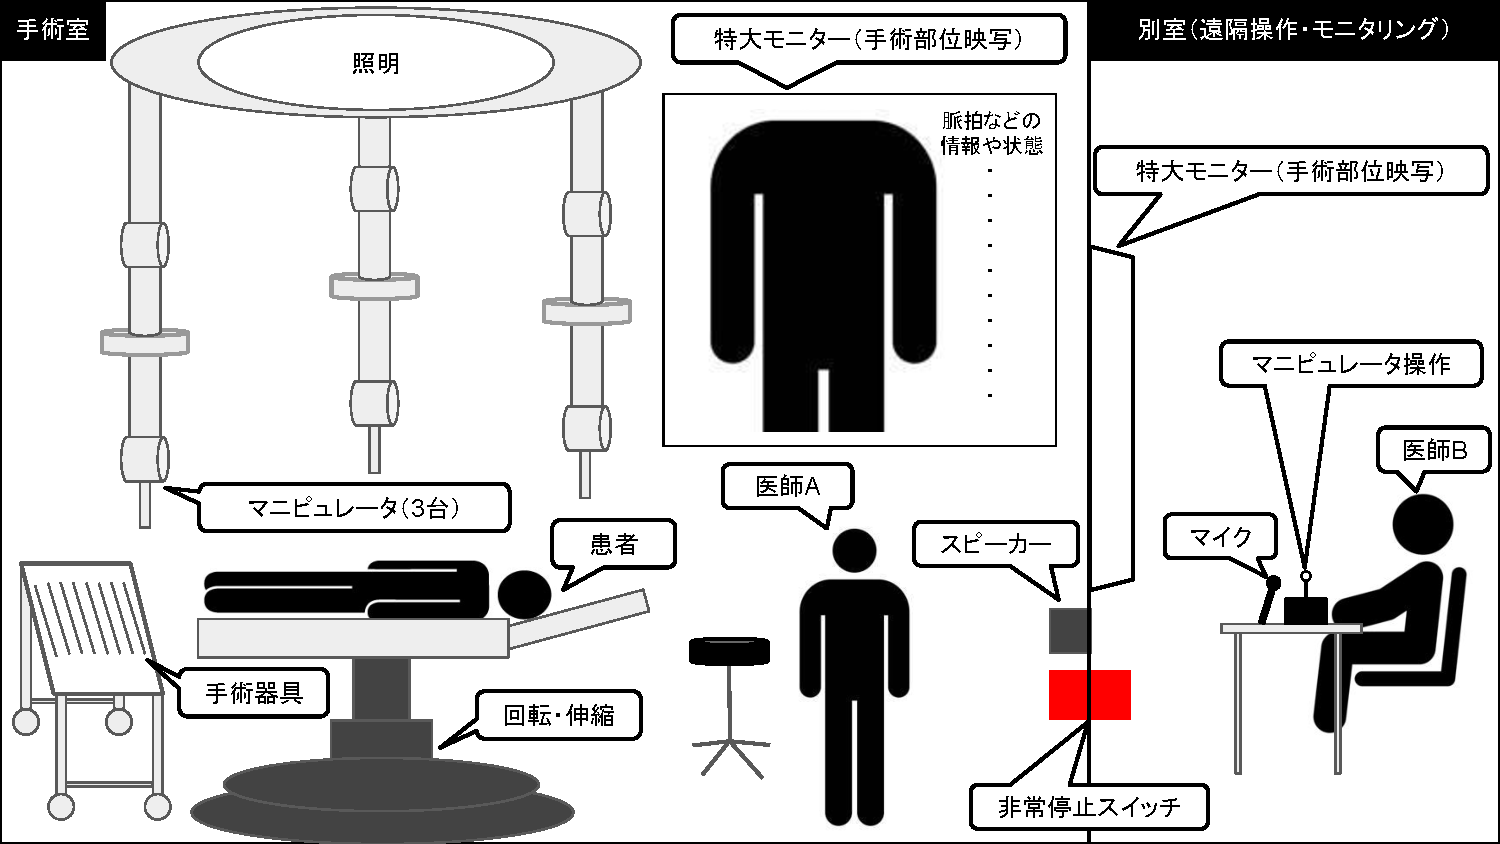
\includegraphics[width=160mm]{a.pdf}
  \caption{私が考える未来(100年後)の手術室}
\end{figure}
\vspace*{-1zh}
\hspace*{5.7zw}近年,AI 技術が目覚ましく発展しており,ロボットが自分の頭で考えて自分で動くというのが
\hspace*{5.7zw}当たり前の世の中となってきている.また,先述の国際ロボット展のDENSOブースの経路計画
\hspace*{5.7zw}手法のように,ロボット同士が互いに干渉せずに,動作することができるようになってきている.\\
\hspace*{5.7zw}よって,未来ではこれらの技術がさらに発展し,複数のロボットが互いに協調して手術ができる
\hspace*{5.7zw}ようになるのではないかと考えられる.上図に示した未来の手術室は,3台のマニピュレータが
\hspace*{5.7zw}自ら手術の計画を立て,実行するというものである.その際,マニピュレータ同士で手術器具の
\hspace*{5.7zw}受け渡しも行っているのではないかと考えられる.さらに,手術の行いやすさを考慮して,マニ
\hspace*{5.7zw}ピュレータ操作側から別のコンピュータへ通信することで,患者が横たわるベッドの高さや向き
\hspace*{5.7zw}も変えているのではないだろうか.AI 技術の他に,近年では画像処理技術が発展している.よっ
\hspace*{5.7zw}て,未来ではモニタリングシステムが大きく向上しているはずである.これは,手術中にリアル
\hspace*{5.7zw}タイムで状態を映し出すだけでなく,次のロボットの動作,触れる場所などを表示できるように
\hspace*{5.7zw}なると考えられる.ただし,私は100年後であったとしても,完全にロボットのみで手術を行う
\hspace*{5.7zw}ことはないと考える.その理由としては,人間が目を見張っていないと不測の事態が起こった際
\hspace*{5.7zw}に対応できないからである.いくら高度なシステムであっても,リスクは少なからず存在するだ
\hspace*{5.7zw}ろう.したがって,手術室には必ず一人の医師は常駐していると考えられる.それに加え,遠隔
\hspace*{5.7zw}操作技術も発展しているため,別室で他の医師がモニタリングしつつ,一部の場面ではマニピュ
\hspace*{5.7zw}レータの操作を手動に切り替えるといったことも行っていると考えられる.なお,2023年1月5
\hspace*{5.7zw}日には,Microsoft社より,たった3秒のサンプルで人の声を再現できる音声合成AI 「VALL-E」
\hspace*{5.7zw}が発表されている.このように,対話と音声のような人間のコミュニケーションに必要な要素に
\hspace*{5.7zw}関するAIも発展している.そのため,今後,人間とロボットが違和感なくコミュニケーション
\hspace*{5.7zw}を取る時代が来ると予想される.これを踏まえ,未来の手術室では人間がロボットに対し,音声
\hspace*{5.7zw}で指示を出して手術を行っていると考えられる.



\newpage

\vspace*{-10zh}

\textbf{{[設問 3]}}\hspace*{1zw}人間の手と全く同じ様に動作する義手が開発できる技術をもっているとする.\\
\hspace*{5.7zw}(3-1) この義手に必要不可欠な機能,性能などを具体的に述べよ.

\begin{itemize}
  \addtolength{\itemindent}{5.4zw}
  \item 感覚フィードバック機能\\
  \hspace*{5.5zw}義手が物をつかむ力や物体の形状,温度などを感じ取り,それを使用者に伝える能力が必
  \hspace*{5.5zw}要不可欠である.これにより,使用者は義手を使って物体を適切に操作できる.\\

  \item 精密なモーターコントロール性\\
  \hspace*{5.5zw}人間の手は非常に複雑な動きを行うことができる.そのため,義手も指の曲げ伸ばしや
  \hspace*{5.5zw}回転など,様々な微細な動きを再現できる必要がある.\\

  \item 耐久性や信頼性\\
  \hspace*{5.5zw}義手は日常生活のさまざまな場面で使用されると考えられるため,頑丈で信頼性が高いこ
  \hspace*{5.5zw}とが求められる.また,雨でも使用できるように防水性が必要である.さらに,耐衝撃性
  \hspace*{5.5zw}も重要である.\\

  \item 自然な見た目\\
  \hspace*{5.5zw}義手が人間の手と見た目が似ていれば,使用者は人目を気にせずに社会生活を送ることが
  \hspace*{5.5zw}できる.\\

  \item 直感的な操作性\\
  \hspace*{5.5zw}使用者が義手を自分の体の一部と感じて,自然に操作できるようにするためのインター
  \hspace*{5.5zw}フェイスが必要である.\\

  \item 高いエネルギー効率\\
  \hspace*{5.5zw}義手は一日中使用されると考えられるため,バッテリー寿命とエネルギー効率が重要に
  \hspace*{5.5zw}なってくると考えられる.長時間使用でき,短時間で充電できるような機能があると良い.\\

  \item  軽量化\\
  \hspace*{5.5zw}義手が重いと,使用者にとっては負担となり,長時間の使用が難しくなる.よって,軽量
  \hspace*{5.5zw}な素材と設計が求められる.\\

  \item カスタマイズ性\\
  \hspace*{5.5zw}使用者の体型や好みに合わせて義手のサイズや形状を調整できる機能が必要である.また,
  \hspace*{5.5zw}義手の動作や感触を自分の好みに合わせて調整する機能もあると良い.\\

  \item 静音性\\
  \hspace*{5.5zw}義手の動作音が大きすぎると,人目につく可能性がある.よって静音性があると良い.\\

  \item 低コスト\\
  \hspace*{5.5zw}多くの人々が利用できるようにするためには,低コストの設計と製造が必要である.\\

  \item  学習能力\\
  \hspace*{5.5zw}義手が使用者の動作パターンを学習し,より効率的に動かせる機能があると尚良い.\\

\end{itemize}
\newpage
\vspace*{-10zh}
\hspace*{4.7zw}(3-2) この場合,健康な腕を切断して義手に変更する事も元の機能を取り戻す意味で\\
\hspace*{8.4zw}医療行為とすることができるはずである.\\
\hspace*{8.4zw}この行為の是非について,技術的・倫理的観点から考えて個人的な意見を述べよ.\\

\hspace*{8.4zw}まず,技術的な観点から考えると,義手に変更する手術が100%安全であるとは考えに
\hspace*{8.4zw}くい.例えば,感染症,出血,医療ミス等による,手術失敗の可能性は常につきまとう.体
\hspace*{8.4zw}の健康というのは,全ての人にとって大切なものである.さらに,腕に関しては,人間の
\hspace*{8.4zw}行動の選択肢をとても広げているため,体の中でも重要度が高いといえる.そのため,い
\hspace*{8.4zw}かにオシャレな義手などの付加価値があったとしても,心理的なハードルはとても高いも
\hspace*{8.4zw}のであると考える.

\hspace*{8.4zw}次に, 倫理的な観点から考える.まず,自分自身を傷付ける行為は正しいのだろうか.い
\hspace*{8.4zw}じめや悩みなどのストレスなどにより,自殺寸前まで自分自身の精神や体を傷つけてしま
\hspace*{8.4zw}う人が存在する.このような人に対して,社会ではホットラインやカウンセラーなどによ
\hspace*{8.4zw}る対策を行っている.このことから,道徳的に自分自身を傷付ける行為は正しくないと考
\hspace*{8.4zw}えられる.確かに,義手を取り付けることによって元の機能を取り戻すことが,医療行為
\hspace*{8.4zw}と見なせる可能性はあるが,過程を考えると健康な腕を切断してしまっている.このこと
\hspace*{8.4zw}は,自分自身を傷付ける行為に当たるといえる.よって,技術的・倫理的観点から見ても
\hspace*{8.4zw}健康な腕を切断し,義手に取り替えるというような行為は容認できない.

\end{document}
